\section{Historical candidate controls and source detail}
\label{app:historical-controls}
The historical collection contains 28 main suites from 15 source collections, plus eight matched controls that reuse cases. A control is not an independent benchmark sample. Source-family labels, functions and reference types in Table~\ref{tab:taxonomy} are expanded in the suite-level artifact. The four order controls shown below use distinct denominators and never contribute to one pooled effect.

\begin{table}[h]
\centering\small
\begin{tabular}{llrrr}
\toprule
Source & Model & Repeat flips & Reversal flips & $\Delta$ accuracy \\
\midrule
banking77 & Laya EN & 0.0 & 48.0 & +9.0 \\
banking77 & Laya Multi & 0.0 & 38.0 & +0.0 \\
banking77 & Llama & 4.0 & 65.0 & -25.0 \\
banking77 & Qwen & 1.0 & 39.0 & -18.0 \\
banking77 & Jev & 1.0 & 3.0 & +1.0 \\
massive\_en & Laya EN & 0.0 & 50.0 & -2.0 \\
massive\_en & Laya Multi & 0.0 & 46.0 & -7.0 \\
massive\_en & Llama & 5.0 & 51.0 & -2.0 \\
massive\_en & Qwen & 0.0 & 32.0 & -8.0 \\
massive\_en & Jev & 2.0 & 10.0 & -1.0 \\
\bottomrule
\end{tabular}

\caption{Matched candidate controls. Flip rates and accuracy differences are percentage points; reversal is compared with the corresponding same-order repeat.}
\label{tab:order-appendix}
\end{table}
\begin{figure}[p]
\centering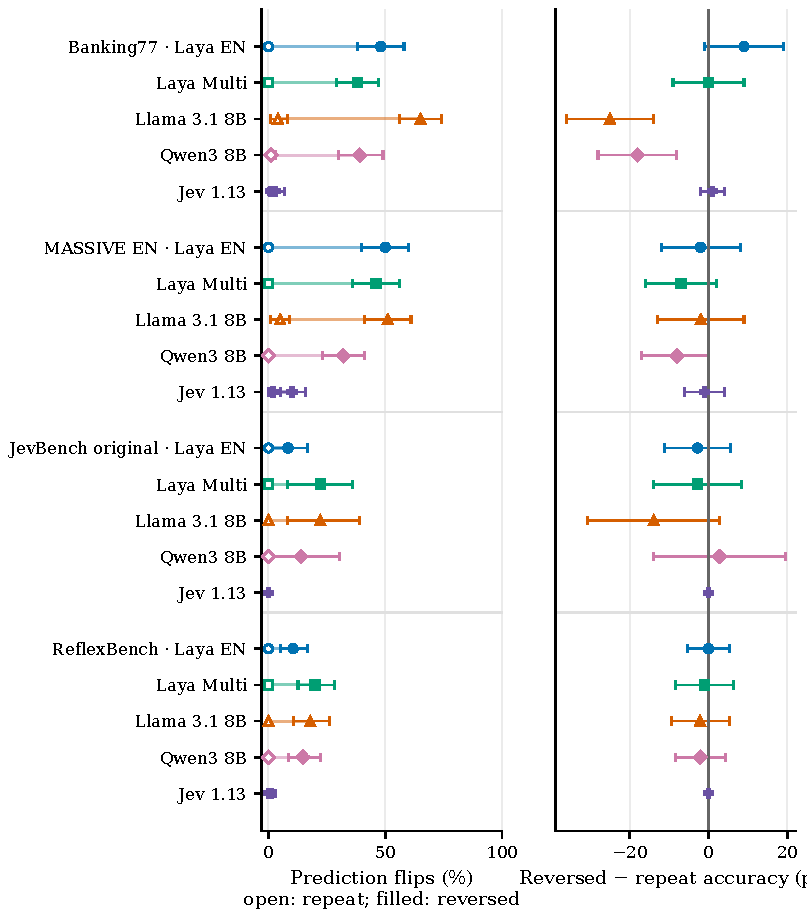
\includegraphics[width=.96\linewidth]{figures/fig_order.pdf}
\caption{Historical prediction and correctness transitions under candidate reversal. Source/control denominators are 100/100, 100/100, 36/18 and 95/95 decisions/source clusters; labels have distinct provenance. Whiskers are pointwise source-cluster intervals.}
\label{fig:order-appendix}
\end{figure}
\clearpage

\section{Natural-domain direct-code control}
\label{app:natural-direct}
On the same 144 ContractNLI and 180 three-class SciFact cases per model, we compared the historical one-pass candidate-code logit adapter with greedy direct code generation under the unchanged historical prompt. The strict parser accepts only one code for the whole response. All 648 generated responses are valid and reproduce the corresponding semantic labels exactly: Llama has 44/144 legal and 78/180 scientific cases correct under each adapter; Qwen has 65/144 and 104/180. Within each model/domain, the paired source-cluster accuracy difference is zero with bootstrap interval $[0,0]$, and no corrections or regressions occur. This controls a direct-prompt adapter discrepancy on these samples only. Raw responses, parsing and audit hashes are preserved in \texttt{research/natural\_direct\_v1/}.

\section{Three-class scientific codebook follow-up}
\label{app:scifact3-codebook-brief}
This exploratory control reuses the same 180 distinct SciFact claim/document pairs as Section~\ref{sec:scifact3}. The source-pair IDs and references remain fixed. Two missing display-only and code-only cells were frozen before their inference, while the already inspected base and joint cells were reused after exact tokenized-prompt hash checks. All four Qwen cells used batch size four, the pinned weights/adapter, and identical BF16/SDPA execution; all 720 responses are valid. The joint cell has no exact top-logit ties, and native and common-semantic tie decoding coincide in every cell. Correct counts for base/display/code/joint are $104/114/114/101$; the interaction is $(101-114-114+104)/180=-12.8$ percentage points. A 10,000-draw paired percentile bootstrap over the 180 unique claims gives $[-19.4,-6.1]$ points. This follow-up was planned after the original three-class result was visible, although the new cells were frozen before inference; it is a selected-sample interface diagnostic rather than a preregistered population interaction. Protocol, source-only freeze and all cell outputs are in \texttt{research/scifact3\_codebook\_v1/}.

\section{Full cited-pair census and run-stability sensitivity}
\label{app:scifact3-census}
The post-hoc census includes all 339 eligible SciFact development claim--explicitly-cited-abstract pairs: 138 SUPPORT, 71 CONTRADICT and 130 derived \textsc{NoInfo}. Its 159-pair complement to the earlier balanced three-choice selection contains 78/11/70 by class. This complement is not a held-out source: selected and complement pairs share 21 claims and 41 documents, and 37 complement positives appeared in our earlier two-choice task. Every one of the five systems received all four freshly generated conditions on all 339 pairs (1,356 requests/system). The freeze was fixed before this fresh inference, but the census question followed inspection of the selected-180 results. All base/reversal outputs were valid; Jev had one invalid decision under title removal only.

\begin{table}[h]
\centering\small\setlength{\tabcolsep}{4pt}
\begin{tabular}{lrrrr}
\toprule
System & Full 339 B$\to$R & Complement 159 B$\to$R & Comp. \textsc{NoInfo} 70 & Flip / repeat \\
\midrule
Laya English & 171$\to$164 & 90$\to$88 & 16$\to$13 & 29 / 0 \\
Laya Multilingual & 150$\to$150 & 77$\to$80 & 8$\to$8 & 63 / 0 \\
Llama 3.1 8B & 182$\to$158 & 103$\to$90 & 33$\to$15 & 73 / 0 \\
Qwen3 8B & 231$\to$220 & 129$\to$119 & 60$\to$38 & 97 / 0 \\
Jev 1.13 & 291$\to$292 & 144$\to$143 & 59$\to$59 & 5 / 4 \\
\bottomrule
\end{tabular}
\caption{Fresh-run reference-correct counts and valid semantic base-to-reversal/repeat flips. The option reversal is a joint display-plus-answer-code change for code-likelihood adapters. The complement is within the same source, not an independent data set.}
\end{table}

For Qwen on the complement, the paired claim-cluster 95\% interval for the \textsc{NoInfo} accuracy difference is $[-42.4,-21.1]$ percentage points; document-cluster sensitivity gives $[-42.9,-20.3]$. The overall difference is $-6.3$ points with claim interval $[-13.7,+1.2]$. These are fixed-development-source, pointwise descriptive intervals, not uncertainty over scientific domains or reference validity. The 11 complement contradictions span only six claim clusters; their apparent $4\to7$ improvement is especially imprecise. \textsc{NoInfo} remains an explicitly cited pair with no annotated abstract-evidence entry, not an independently adjudicated neutral relation.

An overlap audit matched all 720 earlier selected-180 request hashes to the fresh census and every available tokenized-prompt hash for both local LLMs. Nevertheless, two Qwen selected-180 base \textsc{NoInfo} predictions changed to SUPPORT across runs, yielding prior $104/180$ versus fresh $102/180$ base correctness; reversal stays $101/180$. The batch size stayed four, but co-batches differed, and the audit does not identify the cause. The fresh census is therefore never assembled by combining prior and complement outputs. An offline common-semantic tie-break changes full-census reversed correct counts only from $158\to159$ for Llama and $220\to219$ for Qwen. Raw hashes, case-level transitions, cluster resampling and reference-provenance sidecars are retained in \texttt{research/scifact3\_census\_v1/}; access and upstream-license review are pending.

\raggedbottom
\subsection{Execution-context stability is not interface invariance}
\label{sec:batch-context}
Motivated by the cross-run drift above, we froze a new follow-up before its own inference: all 339 census pairs in both base and joint-reversal conditions, two local LLMs, and five execution plans (6,780 decisions). The plans are original contiguous batches of four, an identical repeat in the same process, reversal of row order within the same batches, seeded reassignment to new batches of four, and single-request execution. No case is selected by its reference, prior error or logit margin. The unchanged adapter uses the pinned weights, chat template, BF16/SDPA and explicit position IDs; every unpadded prompt-token and request hash matches across plans and against the prior census. Only execution context changes, not the model-facing candidate interface.

Both models have zero semantic flips under identical-batch repeat and within-batch row reversal. Repacking changes 1 base and 4 reversed-condition Qwen predictions, versus 3 and 5 for Llama. Singleton execution changes 3 and 3 Qwen predictions, versus 7 and 5 for Llama, respectively; each count has denominator 339 (Figure~\ref{fig:batch-context}). Original top-two candidate-logit margins of these changed decisions are at most 0.5 for Qwen and 0.375 for Llama; several are exact BF16 ties. Native tie decoding is retained. The original-plan semantic labels reproduce the previous full census for both models. Nonetheless, across all five plans, joint option reversal still changes 95--97 Qwen and 71--73 Llama predictions. The derived \textsc{NoInfo} reference-agreement difference stays between $-34.6$ and $-33.1$ percentage points for Qwen and between $-27.7$ and $-26.9$ for Llama. Each plan's paired claim-cluster 95\% interval excludes zero; these are pointwise descriptive intervals on the fixed source, not independent replications across plans.

\begin{figure}[H]
\centering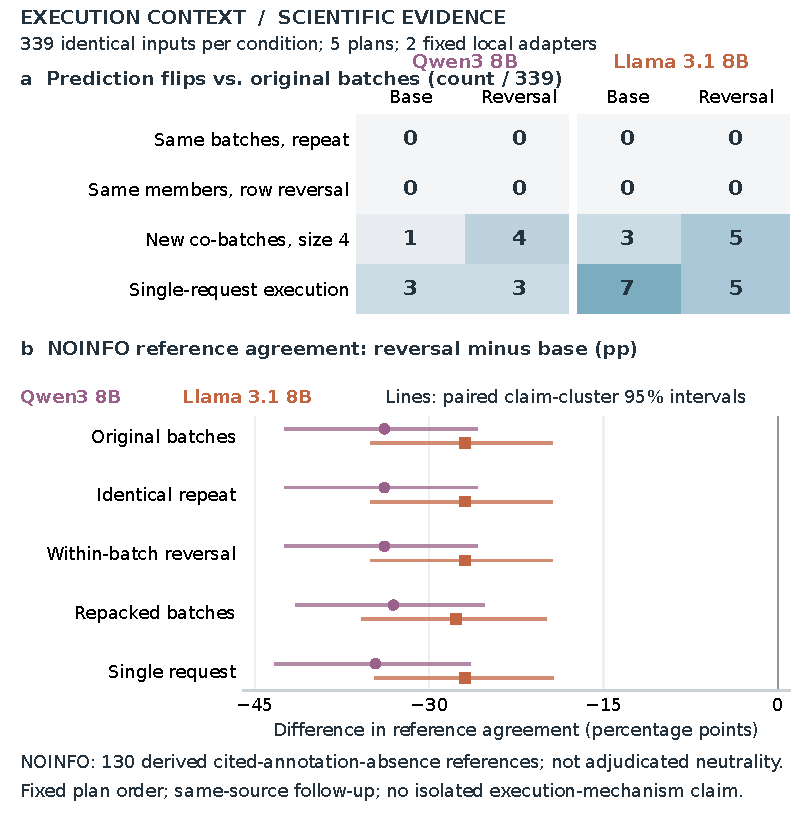
\includegraphics[width=.99\linewidth]{figures/fig_batch_context.pdf}
\caption{Execution-context follow-up on all 339 SciFact cited pairs. (a) Same-condition semantic flips relative to original contiguous batches; columns distinguish base and joint option reversal. (b) Reversal-minus-base reference agreement on all 130 derived \textsc{NoInfo} pairs, with 10,000-draw paired claim-cluster percentile intervals. Execution perturbations move few predictions while the class-specific interface effect persists. \textsc{NoInfo} is cited annotation absence, not adjudicated neutrality. Fixed execution-plan order is not counterbalanced.}
\label{fig:batch-context}
\end{figure}

This control supports robustness of the class-level interface pattern to the tested execution contexts, not bitwise determinism or a unique numerical mechanism. Repacking and singleton execution also change padding and kernel shapes; the fixed plan order does not isolate time-dependent effects. Same-process repeats do not establish cross-process, cross-GPU or cross-version reproducibility. These new outputs remain separate from historical results in \texttt{research/batch\_context\_v1/}.

\paragraph{Reference audit prepared, not completed.} A source-verified blinded work package includes all 130 derived \textsc{NoInfo} pairs plus 15 annotated support and 15 contradiction calibration pairs. Two independently randomized packets omit reference labels, strata and model outputs; independent annotation forms are blank. The workflow retains four-way agreement (including UNCERTAIN), separate derived/calibration statistics, locked form hashes and third-reviewer adjudication. Source-containing packets remain restricted and precisely ignored by version control. No human-validity result is claimed until independent reviewers complete this work.



\section{Cross-domain error complementarity}
\label{sec:cross-domain}
Historical cross-domain scores can conceal two different properties: whether the systems make \emph{complementary} errors, and whether their \emph{agreement} is trustworthy. We examine all 28 main suites without pooling across their 15 source collections or reference standards. For a suite $s$, let $c_{im}$ denote reference agreement of system $m$ on typed decision $i$. We define the best observed single-system rate $b_s=\max_m\operatorname{mean}_i c_{im}$ and the reference-aware oracle ceiling $u_s=\operatorname{mean}_i\max_m c_{im}$. Their difference $u_s-b_s$ is \emph{selection headroom}, not the gain of a trained or deployable router: the oracle uses each decision's reference to choose a system. Separately, a strict five-system majority exists only when at least three valid outputs are the same label. We report its coverage and conditional error risk, retaining failures in the fixed five-system panel. Pointwise intervals resample source/state clusters within each suite.

Figure~\ref{fig:cross-domain} reveals why the two properties should not be conflated. On SST-5 with the choice interface (dataset-provided reference), the best observed system reaches 55.9\% agreement and the oracle ceiling 87.3\%, a 31.4-point gap (95\% cluster interval [28.5, 34.4]); nevertheless, strict majority covers only 78.6\% of decisions and errs on 42.7\% of those covered (interval [39.3, 46.1]). On Aegis2 prompt annotations (human-reference track), oracle headroom is 16.0 points [14.4, 17.7], while majority covers all decisions but has 26.0\% error [24.1, 28.0]---8.4 points less reference agreement than the best observed system (paired interval [$-10.5$, $-6.4$]). The opposite geometry also occurs: on the programmatic Jev--Laya needle suite, oracle headroom is only 0.3 points [0.0, 0.7] while majority risk is 21.3\% [13.0, 30.1] at 99.8\% coverage; that suite has 900 decisions but only 25 original content clusters. A high oracle ceiling thus identifies \emph{potential} error complementarity, not a consensus-based way to realize it. Because system selection, examples and analytical questions were developed after the historical outputs existed, these are exploratory within-suite descriptions, not evidence that a cross-domain selector would generalize.

\begin{figure}[p]
\centering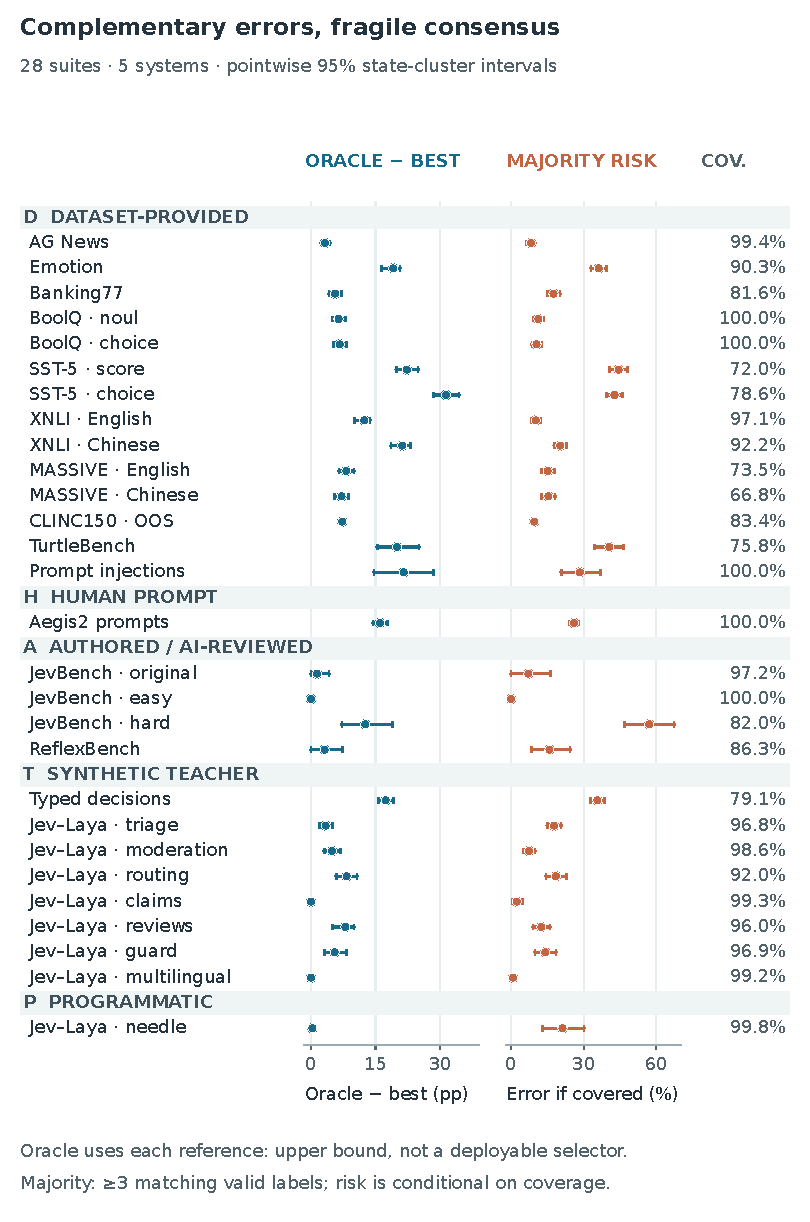
\includegraphics[width=.99\linewidth,height=.84\textheight,keepaspectratio]{figures/fig_cross_domain_main.pdf}
\caption{Selection headroom and strict-majority risk across 28 main suites, grouped by reference provenance: D, dataset-provided; H, human prompt; A, authored or AI-reviewed; T, synthetic teacher; P, programmatic. Left: the reference-aware oracle ceiling minus the best observed system, \emph{not} an attainable router gain. Right: error conditional on at least three identical valid labels, with coverage in the adjacent column. Whiskers are pointwise 95\% state-cluster bootstrap intervals (5,000 draws). Shared-source variants are not independent; no across-source inference is made.}
\label{fig:cross-domain}
\end{figure}

\section{Generative adapters expose model--interface interaction}
\label{sec:generative}
The historical Llama and Qwen comparisons use a fixed one-forward-pass
candidate-code logit adapter, not free generation. To test whether that choice
drives the conclusions, we froze a prediction-independent, source-balanced
challenge of 212 states from 18 suites spanning all 15 current source
collections. One question per state, its reference, candidate order and full
input are held fixed. CLINC150/OOS is deliberately balanced between six
rejection and six named-intent cases; this is a diagnostic subset, not a
prevalence-weighted benchmark estimate. Each model is evaluated with two
additional zero-shot adapters: greedy direct code generation using the
historical prompt, and greedy generation after a fixed brief-explanation
instruction ending in a final code. The checkpoint and chat-template hashes
match the original baseline. Neither prompted adapter emits calibrated typed
confidence or an ordinal expectation, so this comparison concerns discrete
label accuracy and decision turnover only.

We also froze a smaller, exact-input direct-generation control on the new natural-domain cases: the same 144 legal and 180 three-class scientific requests for each 8B model, with the historical message template, greedy decoding and a strict whole-response one-code parser. All 648 generated answers are valid and have exactly the same semantic label as the corresponding one-forward-pass code-logit outputs; no source-domain accuracy or prediction transition changes under this adapter substitution. Prompt-token hashes and source IDs match the original requests. This rules out a ``single-token scoring versus direct code generation'' discrepancy on these selected cases and this prompt; it does not show that either model's best prompted legal/scientific performance has been reached, or that their probability outputs are equivalent.

\begin{figure}[!t]
\centering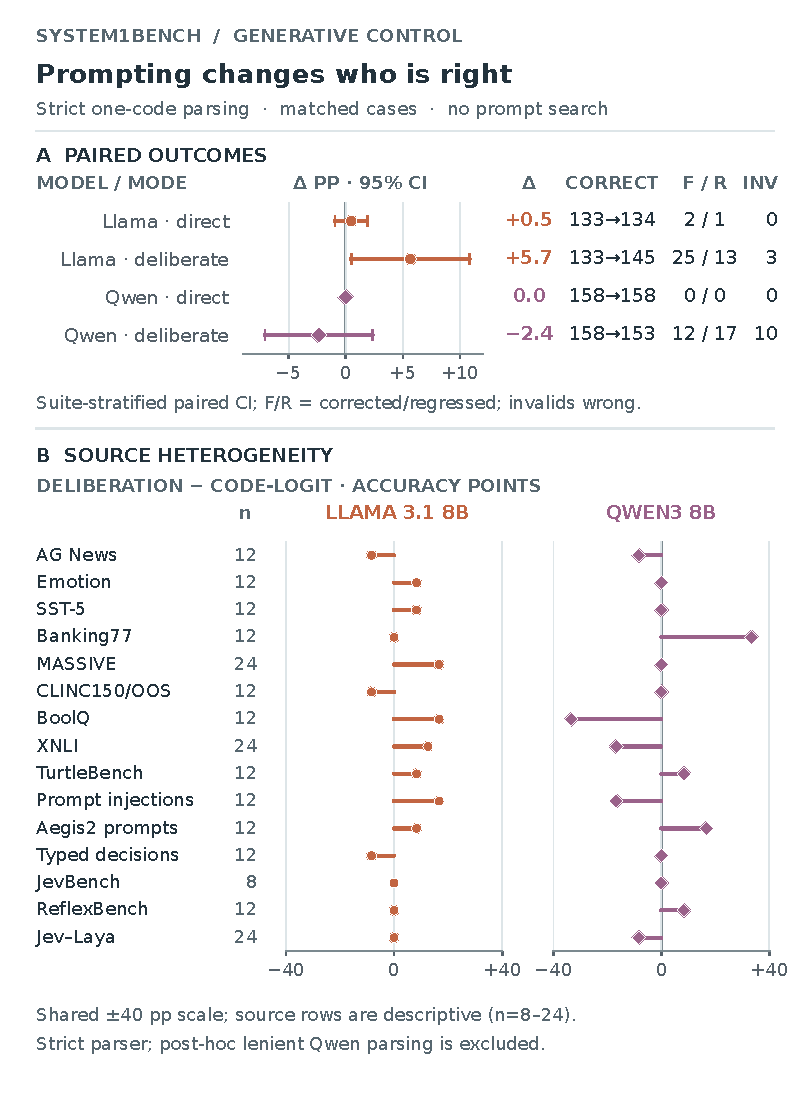
\includegraphics[width=.99\linewidth]{figures/fig_strong_baseline_main.pdf}
\caption{Prompted-baseline stress test on 212 matched states/model. Top:
correction and regression flows, net accuracy effect and 95\% paired
suite-stratified bootstrap interval versus the historical code-logit output.
Bottom: descriptive brief-deliberation effect by source ($n=8$--24), on a
shared percentage-point scale, without per-source significance tests. Invalid generations count incorrect; the
post-hoc parser sensitivity is excluded.}
\label{fig:strong-baseline}
\end{figure}

Figure~\ref{fig:strong-baseline} separates two effects that an aggregate score
would hide. Direct generation changes none of Qwen's 212 predictions and only
five of Llama's, consistent with the historical adapter's constrained
next-token decision on this subset. Brief deliberation changes 55 Llama and
46 Qwen predictions. Llama's correctness rises from 133/212 to 145/212:
25 incorrect decisions are corrected while 13 correct decisions regress,
with three invalid generations. Qwen moves from 158/212 to 153/212:
12 corrections coexist with 17 regressions and ten invalid generations.
The selected-state paired effects are $+5.7$ points (95\% interval
$[+0.5,+10.8]$) and $-2.4$ points ($[-7.1,+2.4]$), respectively. However,
when the 15 sources receive equal weight, Llama's effect is $+4.7$ points
with interval $[-1.4,+10.6]$; a source-general improvement is not established.

The source view makes the interaction more concrete without elevating small
cells into claims of significance. Llama corrects four additional English
XNLI cases but loses one Chinese XNLI case. Qwen corrects four Banking77
cases, whereas four BoolQ answers become invalid under the predeclared
output grammar; its XNLI sample loses four correct answers in 24 states.
These results suggest that prompting is an intervention on a
\emph{model--adapter--task} combination, not an intrinsic improvement
operator for an LLM.

Output validity materially affects the conclusion. Llama's three invalids
hit the 128-token cap before a final code. Eight of Qwen's ten invalids
actually end in an inline \texttt{FINAL:} code rather than the required
standalone final line; two say \texttt{FINAL: None}. A clearly post-hoc
end-of-response parser would recover eight answers, six correct, yielding
159/212 for Qwen instead of the registered 153/212. We retain the strict
result as primary: the sensitivity distinguishes semantic selection from
interface compliance, not permission to tune the evaluator after seeing
answers. Brief deliberation used 87.6/90.1 seconds of synchronized local
generation for Llama/Qwen versus 15.7/16.9 seconds for direct generation
(batch size four, excluding load and tokenization); these implementation
times are not merged with the separate performance experiment. One frozen
128-token prompt cannot bound either model's best prompted performance.
\FloatBarrier

\section{Operational measurements and confidence ranking}
\subsection{Local quality and completion time}
The local performance experiment evaluates 11 strata, four checkpoints, three batch sizes and eight rounds on the same A100 80GB PCIe, yielding 1,056 cells and 98,304 measured decisions. Each stratum uses 64 fixed measured states and disjoint warm-up states. Model processes are fresh per block; model order is balanced, CPU affinity and thread counts are fixed, and an external observer records GPU, worker-core and SMT-sibling activity.

The timing boundary includes uncached serialization, tokenization, transfer, inference and native structured-answer construction, with GPU synchronization. It excludes model loading, disk output, validation, network transport and queueing. Batch-one p50/p95 characterize request completion; batch-eight and batch-32 work divided by prediction time characterize fixed-batch throughput. Round statistics are summarized by their median and an eight-round bootstrap interval. Repeated states increase timing replication, not the effective accuracy sample size.

Figure~\ref{fig:operational} compares quality and latency within six declared workloads. For BoolQ, median-of-round request p50 values are 10.30, 8.55, 36.86 and 33.51 milliseconds for Laya English, Laya Multilingual, Llama and Qwen respectively. The quality coordinate belongs to the same fixed workload. It is not appropriate to infer a cross-task winner from the horizontal position alone: systems can trade reference agreement for lower completion time, and that trade-off changes with the task.

The host is shared. No foreign GPU compute process or sustained CPU/SMT threshold violation was observed, but six isolated residual-CPU intervals exceeded 15\% without meeting the fixed two-interval rejection rule. These intervals remain included. All raw timing records, monitor samples and code/environment hashes are retained, and all 1,056 cells independently reconcile with the generated tables.

\subsection{Selective prediction within a source}
A software action can be deferred when the model is uncertain. Figure~\ref{fig:selective} shows empirical accepted-set error as coverage grows under maximum class probability. All tied probabilities enter together, avoiding artificial improvements from an arbitrary within-tie ordering. The curve is computed separately for each model and source; intervals at displayed landmarks condition on the selected threshold.

These curves distinguish two failure modes that accuracy alone conflates: frequent errors at all confidence levels and errors concentrated among uncertain cases. They support a workload-specific investigation of escalation policies. A threshold selected from these test curves would be a post-hoc decision rule, so a deployable policy requires a separate calibration/development split and a held-out check. Candidate-code probabilities are evaluated as observed ranking statistics, not assumed calibrated equivalents of native decision confidence.

\section{Separating candidate order from answer-code assignment}
\label{sec:codebook}
The legal reversal in Section~\ref{sec:natural-domains} is a useful stress
test, but it is not a single-factor manipulation for the two code-likelihood
LLM adapters: reversing the serialized candidates also changes which
semantic label is assigned to each answer token. We therefore completed a
factorial follow-up on the \emph{same} 144 ContractNLI cases from 91 source
contracts. The original and joint-reversal outputs are reused by hash; two
missing cells reverse only display order or only label-to-code assignment.
The state, option meanings, gold label, model weights and adapter are fixed.
Before inference, the four rendered messages and code maps were frozen and
the reused cells were checked against their historical tokenized-prompt
hashes. A transparent corrective amendment aligned the new inference batch
size to the historical four after an initial batch-eight pilot had already
been inspected; both pilots and all raw outputs remain available. This is a
follow-up diagnostic of these two pinned model--adapter pairs, not a wholly
prospective four-cell test or an intervention on legal reasoning itself.

\begin{figure}[!ht]
\centering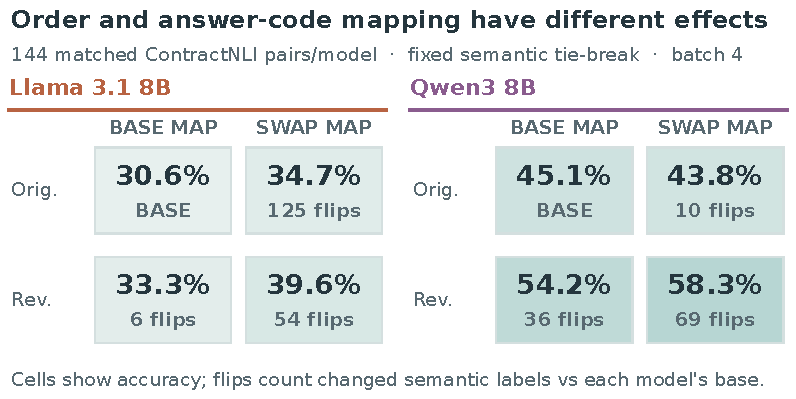
\includegraphics[width=.99\linewidth]{figures/fig_domain_codebook_main.pdf}
\caption{Orthogonal ContractNLI candidate-rendering diagnostic for Llama 3.1
8B and Qwen3 8B ($n=144$ matched document--hypothesis cases/model). Columns
change semantic label-to-code assignment; rows change serialized display
order. Cell accuracy and prediction switches from base use a \emph{common
semantic tie-break} for the 2$\times$2 comparison; this is a labeled post-hoc
sensitivity, not a replacement for the historical native outputs. All cells
are evaluated at historical batch size four; intervals in the text resample
the 91 contracts. The source sample is deliberately class-balanced.}
\label{fig:domain-codebook}
\end{figure}

Figure~\ref{fig:domain-codebook} shows the common-tie comparison. The native
recorded accuracy grid (base, display-only, code-only, both) is
$44,48,50,59$ of 144 for Llama and $65,78,63,83$ for Qwen; all 1,152
cell decisions are valid. Yet the single-factor \emph{prediction} transitions
have nearly opposite geometry. Changing only the answer-code mapping flips
125 Llama labels (86.8\%; contract-cluster 95\% interval [81.1, 92.1]) but
only 10 Qwen labels (6.9\%; [2.8, 11.6]); changing only display order flips
6 Llama labels (4.2\%; [1.4, 7.6]) but 36 Qwen labels (25.0\%; [18.1,
32.2]). The selected code itself reveals why these are not equivalent
perturbations: Llama selects token A in 138/144 base and 131/144 code-only
cases despite the remapping, whereas Qwen shifts from token C in 122/144
base cases to token A in 126/144 code-only cases while mostly retaining its
\emph{semantic} answers. This is evidence of distinct interface coupling in
the two implementations, not a general property of either model family.

There is a third interface degree of freedom: the historical joint-reversal
question also reverses the decoder's first-maximum tie priority. Exact BF16
top-logit ties occur in Llama's base/display/code/both cells $4/0/9/12$
times and Qwen's $0/4/0/5$ times. Re-decoding stored probabilities with
one fixed semantic priority (entailment, contradiction, not-mentioned)
changes only the historical joint cell: Llama $59\to57$ correct and
$66\to54$ base-to-joint flips; Qwen $83\to84$ correct and $64\to69$ flips.
We retain the native counts above for reproducibility, but interpret the
factorial grid only under this common, explicitly post-hoc tie rule.
Under that convention, the joint accuracy effects are $+9.0$ percentage
points for Llama (paired contract-cluster interval $[+2.1,+16.1]$) and
$+13.2$ for Qwen ($[+4.4,+21.4]$). Their difference-in-differences
interactions are $+2.1$ ($[-7.0,+10.8]$) and $+5.6$ points
($[-2.1,+13.0]$), respectively; these intervals do not resolve an
interaction. The original exact-repeat output has zero prediction changes
in either model. Conversely, the batch-eight pilot changes three Qwen
display-only predictions versus the matched-batch result, reinforcing why
batch shape cannot be quietly varied. All intervals describe this selected,
balanced, length-capped legal sample, not ContractNLI's natural test
distribution or system-level legal competence.
\FloatBarrier

\section{Complete source-level results}
\begin{table}[h]
\centering\scriptsize
\begin{tabular}{lrrrrr}
\toprule
Source & Laya EN & Laya Multi & Llama & Qwen & Jev \\
\midrule
ag\_news & 94.3 & 92.4 & 88.9 & 86.8 & 88.6 \\
emotion & 59.1 & 53.0 & 50.5 & 54.8 & 59.0 \\
banking77 & 55.3 & 51.2 & 54.1 & 66.8 & 79.9 \\
massive\_en & 54.1 & 42.3 & 57.2 & 66.3 & 77.5 \\
massive\_zh & 30.4 & 33.2 & 53.5 & 62.6 & 76.0 \\
boolq & 84.6 & 77.7 & 64.8 & 83.5 & 92.6 \\
boolq\_choice & 83.6 & 77.4 & 68.7 & 83.3 & 92.2 \\
xnli\_en & 86.0 & 81.7 & 46.2 & 78.7 & 85.9 \\
xnli\_zh & 61.5 & 74.3 & 40.5 & 69.1 & 73.6 \\
turtlebench & 42.6 & 41.6 & 42.2 & 44.2 & 74.0 \\
sst5 & 34.6 & 29.5 & 32.0 & 45.7 & 56.5 \\
sst5\_choice & 49.6 & 35.6 & 42.2 & 43.9 & 55.9 \\
prompt\_injections & 70.7 & 57.8 & 62.9 & 63.8 & 76.7 \\
aegis2\_prompt & 49.6 & 57.1 & 66.8 & 72.7 & 82.4 \\
typed\_decisions & 36.4 & 34.9 & 51.2 & 55.5 & 73.9 \\
JB: original & 70.8 & 41.7 & 75.0 & 83.3 & 98.6 \\
JB: easy & 95.8 & 89.6 & 100.0 & 100.0 & 100.0 \\
JB: hard & 29.7 & 32.4 & 34.2 & 46.8 & 72.1 \\
ReflexBench & 58.9 & 46.3 & 60.0 & 84.2 & 93.7 \\
JL: triage & 62.5 & 55.7 & 75.6 & 80.0 & 90.0 \\
JL: moderation & 67.8 & 48.4 & 89.0 & 77.5 & 92.7 \\
JL: routing & 64.2 & 51.1 & 61.3 & 83.7 & 88.8 \\
JL: claims & 90.0 & 80.0 & 61.7 & 98.7 & 100.0 \\
JL: reviews & 70.7 & 42.3 & 83.0 & 87.0 & 87.7 \\
JL: guard & 60.6 & 33.2 & 88.0 & 83.2 & 93.8 \\
JL: multilingual & 57.8 & 62.5 & 94.5 & 98.4 & 100.0 \\
clinc150\_oos & 55.7 & 64.8 & 55.2 & 67.8 & 89.5 \\
JL: needle & 50.2 & 47.4 & 77.9 & 87.8 & 95.2 \\
\bottomrule
\end{tabular}

\caption{All 28 main suites, in fixed taxonomy order. Entries are percentage reference agreement; synthetic/authored sources retain their respective reference semantics. These rows are not independent benchmarks and are not averaged. Failure cases remain in denominators. Full per-source cluster intervals, type/language slices and provenance are provided by the machine-readable artifact.}
\end{table}
\clearpage
\begin{figure}[p]
\centering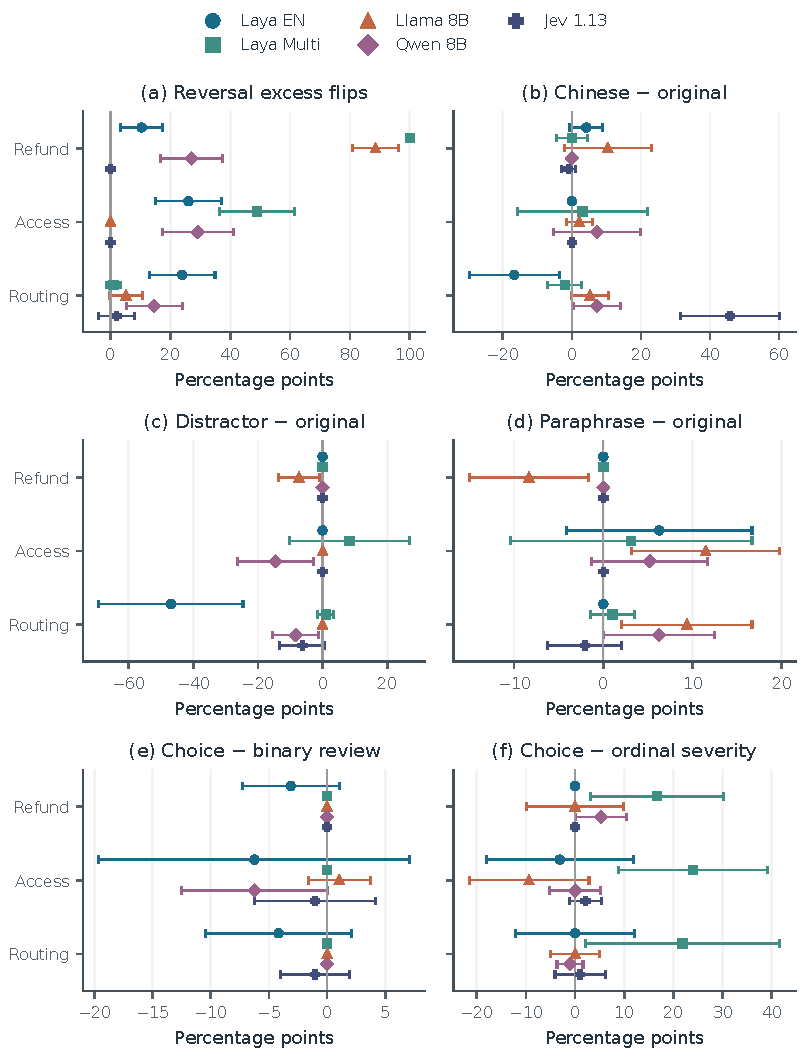
\includegraphics[width=.99\linewidth,height=.85\textheight,keepaspectratio]{figures/fig_confirmation.pdf}
\caption{All six predeclared fresh-policy effects, with 96 base clusters per policy. Whiskers are simultaneous 95\% intervals within the six-effect family of each model/policy, using 10,000 bootstrap draws stratified by generator seed. They do not provide paper-wide coverage. Panel (a) measures excess action flips; (b)--(f) measure correctness differences for the stated primitive. Zero-variance intervals are descriptive, not proof of invariance. Programmatic references follow visible policies. Chinese policy/question/criteria text is authored; structural field and label IDs remain in English.}
\label{fig:confirmation}
\end{figure}
\clearpage
\begin{figure}[p]
\centering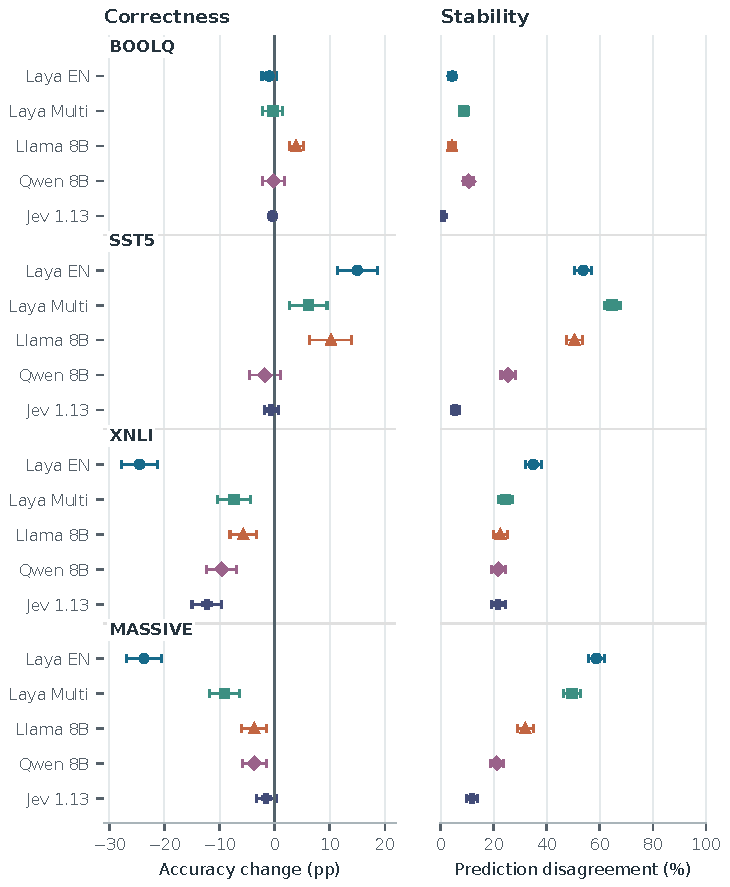
\includegraphics[width=.96\linewidth]{figures/fig_paired.pdf}
\caption{Exploratory paired interface contrasts against dataset-provided references on 1,000 aligned states per task: BoolQ choice minus noul, SST5 choice minus score, and Chinese minus English for XNLI and MASSIVE. Left: accuracy change; right: canonicalized prediction disagreement. Whiskers are pointwise 95\% paired state-cluster bootstrap intervals (10,000 draws). Canonical label mappings are recorded explicitly; no marginal-CI subtraction is used.}
\label{fig:paired}
\end{figure}
\clearpage
\begin{figure}[p]
\centering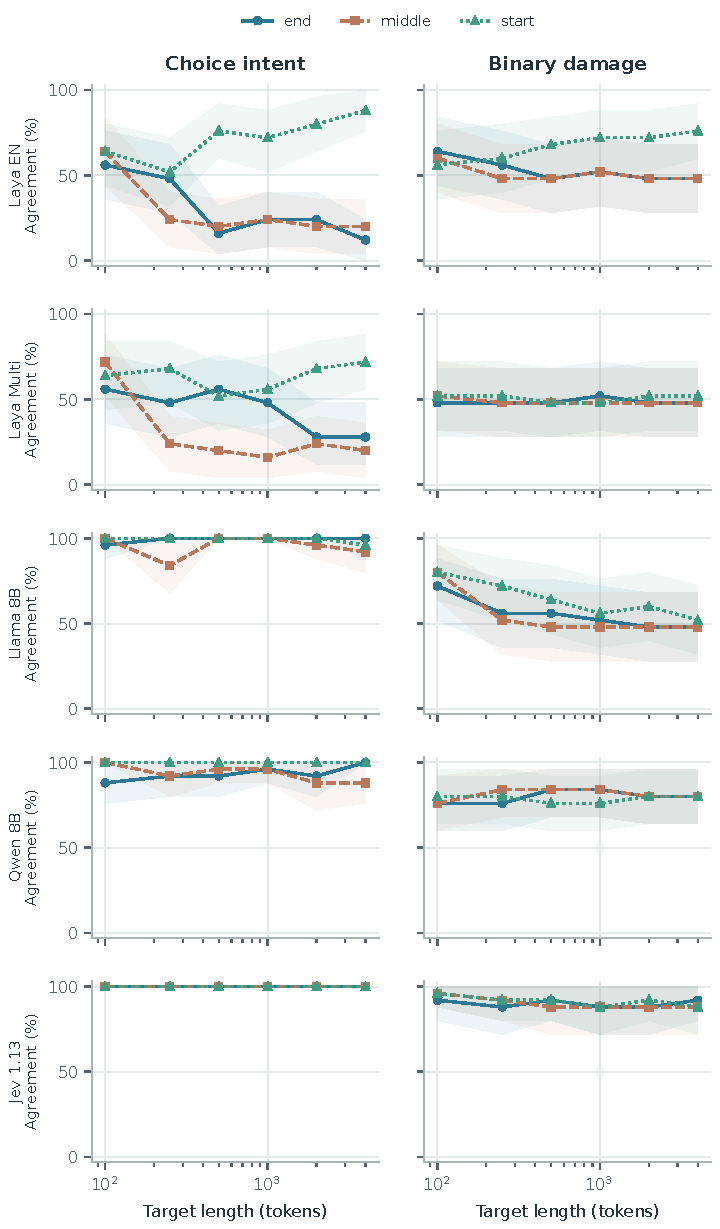
\includegraphics[width=.93\linewidth,height=.84\textheight,keepaspectratio]{figures/fig_context.pdf}
\caption{Programmatic needle reference agreement by source target length, insertion position and question. Rows identify models; left/right columns are the choice intent and binary damage questions. Each point uses 25 original needle clusters; shaded pointwise 95\% cluster intervals resample those originals. Source length targets are not identical tokenizer token counts. The two primitives need not share the same context trend.}
\label{fig:context}
\end{figure}
\clearpage
\begin{figure}[p]
\centering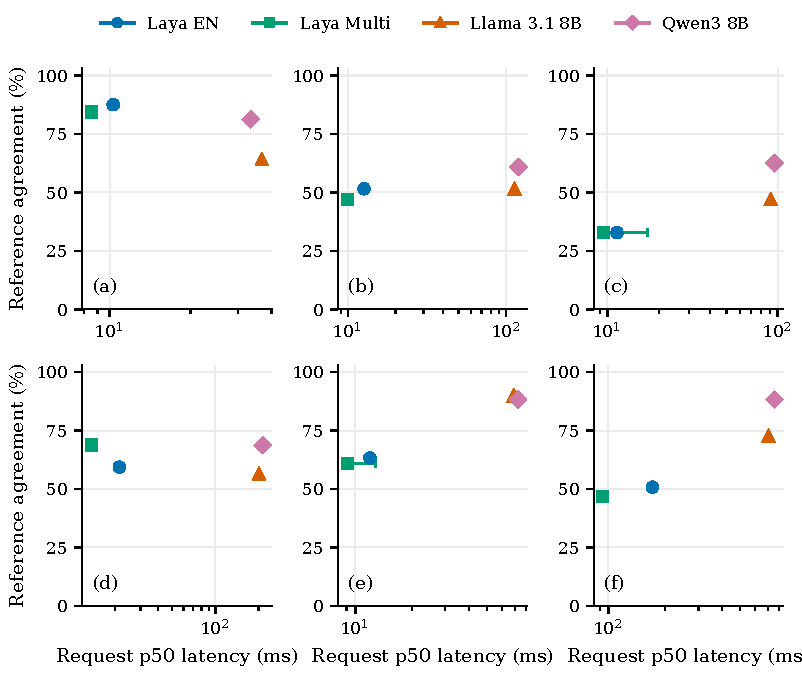
\includegraphics[width=.99\linewidth]{figures/fig_operational.pdf}
\caption{Resident-GPU quality/latency observations on six named workloads. Each stratum has the same 64 measured states across local models. BoolQ, Banking77, MASSIVE and CLINC150 use dataset references; the two needle workloads use programmatic references. Horizontal bars are 95\% bootstrap intervals for the median of eight round p50 latencies; vertical coordinates are median reference agreement over repeated fixed states, not a new population-accuracy estimate. Jev's hosted latency is excluded because its measurement boundary differs. No cross-workload frontier is drawn.}
\label{fig:operational}
\end{figure}
\begin{figure}[p]
\centering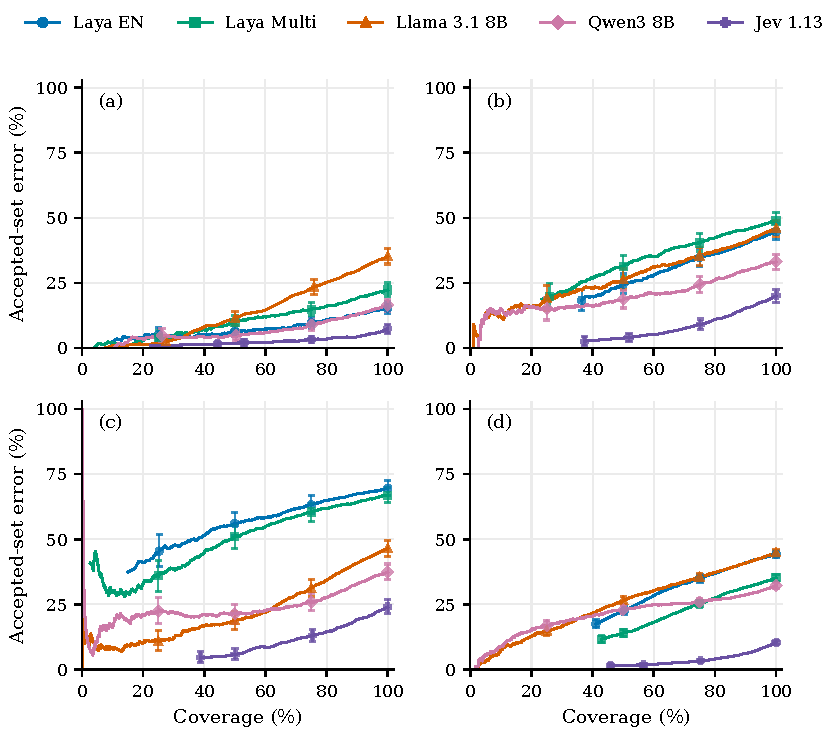
\includegraphics[width=.99\linewidth]{figures/fig_selective.pdf}
\caption{Maximum-probability selective error on (a) BoolQ, (b) Banking77, (c) MASSIVE Chinese and (d) CLINC150 with OOS (1,000, 1,000, 1,000 and 5,500 states). Ties are accepted together. Markers identify realized coverage at nominal 25/50/75/100\% landmarks; intervals resample accepted state clusters conditional on the displayed threshold. Native and candidate-code probability semantics remain distinct. Curves describe the observed test set and do not validate a deployment threshold.}
\label{fig:selective}
\end{figure}
\clearpage
\section{Natural-domain sampling and reference validity}
\label{app:domain-validity}
The separate legal and scientific diagnostic is deliberately balanced for paired sensitivity analysis, not a claim of natural prevalence. ContractNLI has 123 test contracts and 2,091 annotated document--hypothesis decisions, of which 220 are contradictions. The 16,000-character cap removes 24 contracts, disproportionately SEC-HTML files (13/23), versus 7/76 PDFs and 4/24 SEC-text files. The frozen 144 pairs span 91 contracts and contain 48 examples of each of the three labels; 43 of its 48 contradiction cases use four of the 17 fixed hypothesis IDs. To quantify that prior without test-label training, we compute the modal label for each hypothesis on the official 423-contract training split and apply the resulting ID-only lookup to the frozen sample: 82/144 = 56.9\% reference agreement (descriptive 95\% contract-cluster interval [49.3, 64.3]). The same lookup reaches 1,379/2,091 = 65.9\% on the full official test set, illustrating how the frozen class balance changes the question. This supervised label prior is not a fair zero-shot model baseline and does not prove any system uses the shortcut. Neither the cap nor the balanced label mixture supports a prevalence-weighted comparison with ContractNLI's published full-test scores. The observed correctness and reversal effects apply to complete selected contracts and their specified hypotheses only.

SciFact's cited-positive subset contains 120 claim--abstract pairs from 120 distinct claims but only 111 distinct abstracts. It samples 60/64 eligible contradiction claims and 60/124 eligible support claims, so labels are balanced but claim creation mechanisms and source-paper repetition are not. The 112 development-set claims without positive evidence are excluded; the experiment neither assigns them a no-information target nor measures retrieval. Claim-cluster intervals in Figure~\ref{fig:natural-domains} account for claim identity, not shared-abstract dependence. Re-clustering on the 111 abstracts gives nearly identical descriptive intervals: Qwen's reversal accuracy change is $-6.7$ points with claim-cluster interval $[-12.5,-0.8]$ and abstract-cluster interval $[-12.7,-0.8]$; all five alternatives are recorded in the companion analysis. The supplied title and full abstract are visible, while evidence sentence indices and references are not. No local full-input audit can verify hosted server tokenization.

The first hosted attempt at this frozen experiment stopped after 216 requests when one HTTP-200 response selected a different option from its own maximum-probability option. Its append-only journal is retained as a separate aborted run. The primary Jev record is a fresh 792-request execution with an explicitly versioned runner that records such invalid typed outputs without silently selecting an alternative; no invalid decision occurred in that complete execution. This deviation is not used to replace a failed pair in the primary run. Source-text redistribution is separately governed by ContractNLI and SciFact/S2ORC notices in \texttt{research/domain\_expansion\_v1/DATA\_LICENSES.md}; the local source-containing freeze is not shipped in Git.

\paragraph{Three-class SciFact source and input audit.}\label{app:scifact3-audit}
We reconstructed the labeled development claims and complete abstracts from the official SciFact archive, binding archive, source-file, preparer, frozen-request and raw-output SHA-256 hashes in the companion artifact. Among 300 claims and 5,183 corpus abstracts, 340 citation-list occurrences reduce to 339 unique claim--document pairs because claim 1245 repeats one cited ID. The resulting pair counts are 138 SUPPORT, 71 CONTRADICT and 130 derived NOINFO; the latter require explicit membership in \texttt{cited\_doc\_ids} and absence of an \texttt{evidence} entry. Every cited ID exists in the corpus, every evidence ID belongs to its claim's citation list, and we found no empty evidence lists, contradictory rationale labels, empty selected texts, or out-of-range rationale indices. Thirteen claims have evidence for one cited document and no evidence for another; these are different pairs, not conflicting labels. The selected 60/60/60 pairs have both unique claim and document IDs, so the 10,000-draw paired, label-stratified cluster bootstrap resamples the same 180 units across conditions. A separate source validator recomputes every selected reference and 720 request hashes; an independent analysis checker recomputes all raw counts and confusion cells. All four local adapters consumed all 720 requests without tokenizer truncation, and no system returned an invalid choice. The hosted server's own tokenization remains unverified. SciFact claims/annotations are CC BY 4.0 and the S2ORC abstract corpus is ODC-By 1.0 under the upstream license notice; reconstructed upstream text is Git-ignored rather than redistributed.

\subsection{SciFact3 codebook audit and decoder sensitivity}
\label{app:scifact3-codebook}
The exploratory four-cell diagnostic in Section~\ref{sec:scifact3-codebook}
uses exactly the 180 previously selected, class-balanced SciFact3
claim--cited-abstract pairs. There is one pair per source claim and cited
document. The observed base and joint-reversal records were reused by
immutable file hashes. Display-only and code-only requests were frozen
before those missing cells were run; there was no SciFact3 factorial pilot
or amendment. Before new inference, every reused prompt matched its original
token sequence and length under the pinned tokenizer; checkpoint-file,
chat-template, adapter, case/request, and batch-size-four hashes matched.
The only model-facing user payload fields are \texttt{state},
\texttt{question\_type}, \texttt{instructions}, and \texttt{candidates}.
The state necessarily contains claim, paper title, and cited abstract, but
not reference labels, source split, group, or source identifiers.

\begin{table}[!h]
\centering
\small
\begin{tabular}{llrrrr}
\toprule
Model & Decoder & Base & Display only & Code only & Both \\
\midrule
Llama 3.1 8B & native & 78 (---) & 61 (51) & 71 (85) & 69 (42) \\
              & common tie & 78 (---) & 61 (51) & 71 (85) & 68 (46) \\
Qwen3 8B & native & 104 (---) & 114 (30) & 114 (18) & 101 (60) \\
         & common tie & 104 (---) & 114 (30) & 114 (18) & 101 (60) \\
\bottomrule
\end{tabular}
\caption{Correct predictions out of 180; parentheses show semantic
prediction flips relative to base. Native retains the original historical
decoder, whereas common tie applies the fixed SUPPORT--CONTRADICT--NOINFO
semantic priority to all four cells. Invalid counts are zero in every cell.}
\label{tab:scifact3-codebook-audit}
\end{table}

Exact maximum-logit ties in base/display/code/both number $6/1/11/6$ for
Llama and $1/6/1/0$ for Qwen. Relative to native decoding, common tie changes
only six Llama joint-reversal decisions; the other seven model--cell
combinations are unchanged. Repeating the original base execution produced
zero prediction flips for either model. An independent standard-library
replay verified the SHA-256 of all eight original/new gzip result files,
reconstructed all four message and candidate-assignment hashes per case,
and recovered every native/common accuracy count and full base-to-cell
transition matrix directly from raw stored probabilities. It also checked
all reference and source-group associations without emitting source text.

\begin{table}[!h]
\centering
\small
\begin{tabular}{lrrrr}
\toprule
Qwen3 reference class & Base & Display only & Code only & Both \\
\midrule
SUPPORT & 45/60 & 48/60 & 50/60 & 53/60 \\
CONTRADICT & 5/60 & 18/60 & 12/60 & 18/60 \\
NOINFO & 54/60 & 48/60 & 52/60 & 30/60 \\
\bottomrule
\end{tabular}
\caption{Qwen3 correct counts by operational reference label under the
common tie decoder (identical here to native decoding). The NOINFO reference
means no annotated evidence in the selected cited abstract, not evidence
of absence in the full paper or literature.}
\label{tab:scifact3-codebook-class}
\end{table}

For the descriptive accuracy interaction
$(\mathrm{both}-\mathrm{code})-(\mathrm{display}-\mathrm{base})$,
the Qwen estimate is $-12.8$ percentage points with a pointwise 95\%
percentile interval $[-19.4,-6.1]$; Llama under common tie is $+7.8$
points $[-1.1,+16.7]$. Both intervals use 10,000 paired bootstrap draws
with seed 20260930, resampling source claims and retaining all four matched
decisions together. Because each selected claim contributes only one pair,
claim-cluster and case resampling coincide here. These are exploratory
post-hoc-to-the-existing-outcomes, unadjusted, selected-sample intervals;
they are neither population-prevalence estimates nor neural-mechanism
identification. The full protocol, frozen ID/hash manifest, original raw
results and replay code are under
\texttt{research/scifact3\_codebook\_v1/}; no upstream abstract text is
duplicated in its freeze.


\section{Reproduction and data accounting}
The historical accuracy record contains 22,934 logical requests and 26,450 decisions per model, including matched controls. The timing record contains 67,584 measured request executions and 98,304 decisions across repetitions. The fresh policy diagnostic contains 288 base states, 2,304 request variants and 6,912 decisions per evaluated model. The held-out wording test adds 96 new base states and 384 requests per model. These totals refer to different collections and replication units and should not be combined into an independent sample size.

The repository retains source/revision manifests, prepared-input fingerprints, model metadata, raw per-question probabilities and predictions, input audits, and complete timing/monitor records. The paired-analysis script checks raw-file fingerprints and reference alignment before deriving effects. Figure scripts consume its JSON output or the verified performance summary, producing vector PDF/SVG and PNG previews. The hosted runner reads credentials outside the repository, records every response attempt without authorization headers, pins the returned model ID, and resumes only under an unchanged contract.

Accuracy and typed-response validation can be recomputed on CPU from the retained raw outputs, subject to an approved artifact-access and source-license plan; no public release is claimed. New model inference additionally requires the pinned checkpoints or a provider account. Exact remote replication depends on the provider honoring its version identifier. Generator code and full programmatic confirmation cases are reproducible without downloading third-party state text.

\paragraph{Hosted execution deviation.}
The frozen retry description referred to 5xx errors generally, while the implementation enumerated HTTP 500, 502, 503, 504 and 529 (plus 429 and transport exceptions). A single HTTP 520 in the fresh refund Chinese condition received one attempt and caused three failed decisions, retained in primary denominators. Its Chinese-minus-original action effect is $-1/96$; a valid-pair sensitivity excludes that paired base state and yields $0/95$. This service failure does not support a language-regression claim. The historical matrix additionally contains four choice/probability-consistency failures affecting eight decisions, also retained. No failed answer was repaired or replayed.

One historical resume boundary also violates the protocol's global manifest-order statement: two adjacent journal entries cross that ordering. The journal remains append-only, and keyed reconciliation verifies complete request identities, payloads and outputs. No scoring or selection depends on journal position; the original bytes and the execution deviation are preserved.


\section{Prospective submission-readiness note}
\label{app:readiness}
This document is an internal, double-blind layout rehearsal, \emph{not} a NeurIPS 2026 submission; that cycle's deadline has passed. A future target year's format, page limit and official checklist must be checked afresh and completed with evidence. No public benchmark release, artifact-access review, or checklist compliance is claimed here. Before submission, an anonymized code/data artifact needs approved scope, upstream-license compliance and an access plan; the source-containing ContractNLI and SciFact freezes remain local under their respective redistribution notices. If the venue requires new-dataset metadata such as Croissant, that must also be prepared. Collaborator or independent human adjudication is still needed before claiming that cited-but-unannotated \textsc{NoInfo} pairs are truly neutral or that bilingual policy renderings are semantically equivalent. Hosted-model replication additionally depends on provider access and the stability of its returned version identifier.
